\documentclass[11pt]{article}

% ============================================================================
%  토큰-세이퍼 (한국어판). 빌드: tectonic vs-token-safer.ko.tex
%  한국어 조판은 kotex(xetexko) — 어절 띄어쓰기/줄바꿈을 한국어 규칙대로 처리.
%  도표: figures/*.pdf  (python figures/build.py 로 SVG에서 재생성)
% ============================================================================

\usepackage{kotex}
\setmainhangulfont{Malgun Gothic}
\setsanshangulfont{Malgun Gothic}
\usepackage{microtype}
\usepackage[margin=1in]{geometry}
\usepackage{amsmath,amssymb}
\usepackage{booktabs}
\usepackage{graphicx}
\usepackage{xcolor}
\usepackage{hyperref}
\usepackage{url}
\hypersetup{colorlinks=true, linkcolor=blue!55!black, citecolor=blue!55!black, urlcolor=blue!55!black}
\linespread{1.08}
% 한국어는 \sloppy를 쓰지 않는다(어절 간격이 과도하게 늘어남). 약한 신축만 허용한다.
\setlength{\emergencystretch}{1em}

\title{\textbf{토큰-세이퍼: LLM 코딩 에이전트를 위한, grep 대신 공식 언어 서버\\
인덱스를 강제하는 무전송·토큰캡 코드 검색}}

\author{
  전성민 (Sungmin Jeon)\\
  \texttt{sungmin1505104@gmail.com}
}
\date{2026년 6월}

\begin{document}
\maketitle

\begin{abstract}
코딩 에이전트는 저장소를 도구 호출로 읽으며, 그 결과는 모두 모델이 추론에 사용하는 동일한
컨텍스트 창을 점유한다. 일반적인 도구는 \texttt{grep}이고, 그 출력은 전체가 그대로 삽입된다.

이 방식은 구현은 쉽지만 소비는 비효율적이다. 텍스트 검색은 함수와 같은 이름의 변수, 주석을
구분하지 못하므로 모델이 읽고 폐기해야 하는 결과까지 함께 반환한다. 또한 그 비용은 답의
크기가 아니라 일치한 줄 수에 비례하여 증가한다.

본 논문은 로컬 전용 Model Context Protocol(MCP) 서버이자 명령줄 도구인
\textbf{vs-token-safer}(\texttt{vts})를 제안한다. \texttt{vts}는 자체 인덱스를 구축하는
대신 검색마다 \emph{공식} 언어 서버 --- clangd, Roslyn 서버,
\texttt{typescript-language-server}, pyright --- 로 질의를 전달한다. 모든 답은 본문 없는
간결한 \texttt{file:line} 목록으로 토큰캡된다. 그리고 \texttt{grep} 호출을 훅 계층에서 동일
의미의 캡 호출로 재작성하여 대체를 강제한다.

저장, 임베딩, 네트워크 전송은 일어나지 않는다. 74개 검사 하버스와 수 개월의 단일 개발자
사용 데이터에서, 캡 출력은 원시 인덱스 응답보다 약 $2\times$, 가장 무거운 질의에서는 최대
$10.7\times$ 작았다. 강제 계층은 대형 게임 엔진 트리에서 월 수십만 토큰 규모의 잠재적
\texttt{grep} 트래픽을 흡수하였다. 탐색·참조·이름변경 작업에서 \texttt{vts}는 \texttt{grep}의
더 안전하고 저렴한 대체재이다. 어휘 검색이 여전히 더 적합한 영역도 함께 제시한다.
\end{abstract}

\section{서론}
\label{sec:intro}

에이전트가 낯선 저장소를 열면 가장 먼저 수행하는 작업은 검색이다. 세 질문이 지배적이다.
\texttt{X}가 어디에 정의되는가, 무엇이 \texttt{Y}를 호출하는가, \texttt{Z}는 어디에서 사용되는가.

오늘날 대부분의 에이전트는 세 질문 모두를 \texttt{grep}으로 답하고, 결과를 컨텍스트에 그대로
삽입한다.

이 방식은 편리하지만 두 비용을 동반한다. 첫째는 정밀도이다. 텍스트 검색은 주석과 문자열
리터럴의 일치, 부분 문자열을 공유하는 무관한 식별자, 질의하지 않은 오버로드까지 모두 반환한다.
모델은 이를 읽는 데 토큰을, 폐기하는 데 주의를 소모한다.

둘째는 분량이다. grep 결과의 토큰 수는 답의 크기가 아니라 일치한 줄 수와 함께 전달된 맥락에
비례한다. ``어디에 있는가''라는 질문의 답은 짧은 위치 목록에 불과하다.

언어 서버는 정밀도 문제를 이미 해결한다. LSP(Language Server Protocol)는 정의, 참조, 문서·
작업공간 심볼, 호출 계층, 이름변경 같은 시맨틱 연산을 실제 파서와 타입 해석기 위에서 제공한다.
따라서 참조 질의는 텍스트상 유사어가 아니라 실제 참조 지점을 반환한다.

보고된 결과도 동일한 결론을 가리킨다. 이름변경·타입검사·호출체인 작업에는 LSP가 적합한
백엔드이며, grep으로 약 2천 토큰이 드는 조회가 LSP에서는 약 5백 토큰에 종료된다
~\cite{lsp-medium,semble-hn}. Anthropic은 2025년 말 Claude Code에 네이티브 LSP 지원을
추가하였다~\cite{anthropic-lsp}.

남은 문제는 둘이다. 에이전트가 인덱스를 단지 제공받는 데 그치지 않고 \emph{사용하도록} 만드는
방법, 그리고 인덱스에서 모델 컨텍스트로 무엇을 전달할 것인가이다. 본 논문은 두 문제 모두에
명확한 입장을 취하며, 이를 세 약속으로 정리한다.

\begin{enumerate}
  \item \textbf{공식 엔진을 재사용하고 접착부만 구현한다.} C++·C\#·TypeScript·Python의
  정확한 인덱싱은 어려운 작업이며, clangd·Roslyn·\texttt{tsserver}·pyright가 이를 이미
  수행한다. 토큰 절감 도구는 얇은 LSP-MCP 어댑터여야 한다. 파서 재구현도, 타인의 소스 위에
  얹은 제3자 인덱스도 아니다.

  \item \textbf{질문만이 아니라 답을 캡한다.} 절감은 시맨틱 질의를 던지는 것만큼이나 본문을
  반환하지 \emph{않는} 데서 발생한다. 모든 답은 중복이 제거되고 디렉터리 접두사가 추출된
  \texttt{file:line} 목록이므로, grep-붙여넣기보다 적은 소스가 모델에 도달한다. 프라이버시와
  토큰이 함께 개선된다.

  \item \textbf{대체를 제안이 아니라 강제한다.} 더 나은 도구를 \emph{사용할 수 있는}
  에이전트도 습관적으로 \texttt{grep}을 호출한다. 본 연구는 안전한 단일 \texttt{grep} 호출을
  사전 훅에서 동일 의미의 캡 호출로 재작성하며, 에이전트의 흐름은 유지한 채 우회만 제거한다.
\end{enumerate}

\paragraph{기여.}
본 논문의 기여는 다음과 같다. (i) 공식 언어 서버 넷을 하나의 캡·호출별 루트 도구 표면 뒤에
두는 얇은 LSP-MCP 어댑터(절~\ref{sec:arch}). (ii) 위치만 반환하고 파일별로 묶어 접두사를
추출하는 출력 압축 기법으로, 원시 인덱스 응답 대비 약 $2\times$, 최악 질의에서 $10.7\times$로
측정된다(절~\ref{sec:cap}, \ref{sec:eval}). (iii) grep을 동일 의미의 캡 호출로 재작성하고
grep 습관과 ``선언 전체 편집'' 습관을 정량화·유도하는 훅 계층(절~\ref{sec:enforce}). (iv)
재현 가능한 74개 검사 하버스와, 실제 프로젝트에서 수행한 clangd·Roslyn·\texttt{tsserver}·
pyright 라이브 검증(절~\ref{sec:eval}).

\paragraph{대비되는 설계.}
\emph{Codebase-Memory}~\cite{cbm}는 동일한 토큰 문제를 정반대 방향에서 접근한다. 66개
언어에 걸친 \emph{영속} Tree-Sitter 지식 그래프를 구축하고, 선택적 임베딩 벡터 검색과 로컬
시각화를 추가한다. \texttt{vts}는 그 선택을 각각 반전한다. 저장된 그래프 대신 주문형 공식-LSP
질의, 직접 구현한 파서 대신 컴파일러급 엔진, 임베딩 대신 무전송 원칙이다. 이 대비가 본 논문의
나머지를 구성한다(절~\ref{sec:related}).

\section{배경과 관련 연구}
\label{sec:related}

\paragraph{검색의 중추로서의 grep.}
어휘 검색이 기본 도구인 데에는 타당한 이유가 있다. 빌드가 필요 없고, 파일 형식을 가리지
않으며, 모든 텍스트를 검색한다. 이는 낯선 트리에 막 진입한 에이전트가 요구하는 특성이다
~\cite{yage-grep}.

약점 또한 분명하다. 어휘 검색은 심볼과 부분 문자열을 구분하지 못하고, 출력을 관련성으로
제한하는 장치가 없다~\cite{lsp-medium}. Semble 같은 최신 에이전트 검색 도구는 구조화·중복
제거된 결과를 반환하여 grep 대비 최대 $98\%$ 토큰 절감을 보고한다~\cite{semble-hn}. 본
연구는 grep을 그대로 전달할 것이 아니라 제한하고 보완해야 한다는 교훈을 취한다.

\paragraph{에이전트를 위한 LSP.}
LSP를 코딩 에이전트에 연결하여 텍스트 매칭 대신 시맨틱 탐색과 실시간 진단을 제공하려는 연구가
증가하고 있다~\cite{lsp-medium,anthropic-lsp,hyperagent}. \texttt{vts}는 그 계열에 속하되
강조점이 다르다. \texttt{vts}는 LSP 클라이언트일 뿐 아니라 단단한 출력 캡을 갖춘 강제기이며,
선택적 도구 집합이 아니라 grep을 대체하는 훅을 포함한 드롭인 MCP 플러그인으로 제공된다.

\paragraph{왜 자체 인덱스를 구축하지 않았는가.}
명백한 대안은 Codebase-Memory~\cite{cbm}처럼 시맨틱 인덱스를 직접 구축하는 것이다.
Codebase-Memory는 자체 타입 해석기와 선택적 임베딩을 갖춘 Tree-Sitter 그래프를 저장하고,
31개 저장소에서 양호한 절감을 보고한다. 유능한 설계이다. 그러나 본 연구는 반대 방향을 택하였다.
이유는 셋이다.

첫째, 저장된 그래프는 진실의 두 번째 사본이다. 소스와 어긋나며, 무효화와 재구축이 필요하다.

둘째, 직접 구현한 파서는 두 번째 구현이다. 프로젝트가 실제로 사용하는 컴파일러와 어긋날 수
있으며, 그 경우 에이전트는 빌드와 다른 답을 받는다.

셋째, 임베딩은 데이터가 저장·전송될 표면을 추가하므로, 본 연구가 지키려는 무전송 원칙을
위배한다.

따라서 \texttt{vts}는 시맨틱 데이터베이스를 저장하지 않고, 모든 시맨틱 질의를 빌드 자신의
컴파일러 프런트엔드에 위임하며, 아무것도 전송하지 않는다. 다만 주문형 호출 그래프와 콘텐츠
해시 무효화라는 두 아이디어는 그 연구에서 차용하되, 저장된 그래프가 아니라 일시적 LSP 질의와
작은 로컬 캐시로 구현한다(절~\ref{sec:beyond}).

\section{설계 원칙}
\label{sec:principles}

네 불변식이 \texttt{vts}를 규율하며, 각각을 회귀 하버스가 검사한다(절~\ref{sec:eval}).

\begin{description}
  \item[P1 --- 공식 엔진, 우리 접착부.] 분석은 clangd(LLVM)와 Roslyn 기반 서버(Microsoft)가
  수행하고, 본 연구는 LSP-MCP 어댑터만 구현한다. 소스 위에 제3자 MCP 서버를 재사용하지 않으며,
  파서를 재구현하지 않는다.

  \item[P2 --- 토큰 우선.] 모든 기능은 토큰 이득을 유지하거나 향상시켜야 한다. 출력은
  \texttt{file:line}, 캡, 본문 없음이며, 새 기능은 출력이 캡을 유지함을 보장하는 하버스 검사와
  함께만 도입된다.

  \item[P3 --- 로컬 전용, 무전송.] 네트워크 호출이 없으며, 임베딩·업로드·보고가 없다. 캡이
  본문이 아니라 위치를 반환하므로 grep-붙여넣기보다 적은 소스가 모델에 도달한다. 프라이버시
  논거와 토큰 논거가 일치한다.

  \item[P4 --- 선택이 아닌 강제.] 호출을 잊은 더 나은 도구는 아무것도 절약하지 못한다. 대체는
  grep 호출을 동일 의미의 캡 호출로 재작성하여 훅에서 강제하며, 재작성이 안전하지 않을 때는
  점진적으로 후퇴한다.
\end{description}

\section{시스템 아키텍처}
\label{sec:arch}

\texttt{vts}는 하나의 코어 위에 세 얼굴을 제공한다. MCP 서버는 작고 고정된 도구 집합을
에이전트에 노출한다. 일급 도구 13개와, 잘 쓰이지 않는 관리 연산 9개를 접은 단일
\texttt{vts\_admin} 도구로 구성된다. \texttt{vts} CLI는 동일한 연산을 셸에 노출한다. 훅
집합은 grep 계열 호출을 가로채 재작성한다.

그림~\ref{fig:layers}은 구성 요소의 적층을, 그림~\ref{fig:arch}은 단일 요청의 경로를 보인다.

\begin{figure}[h]
\centering
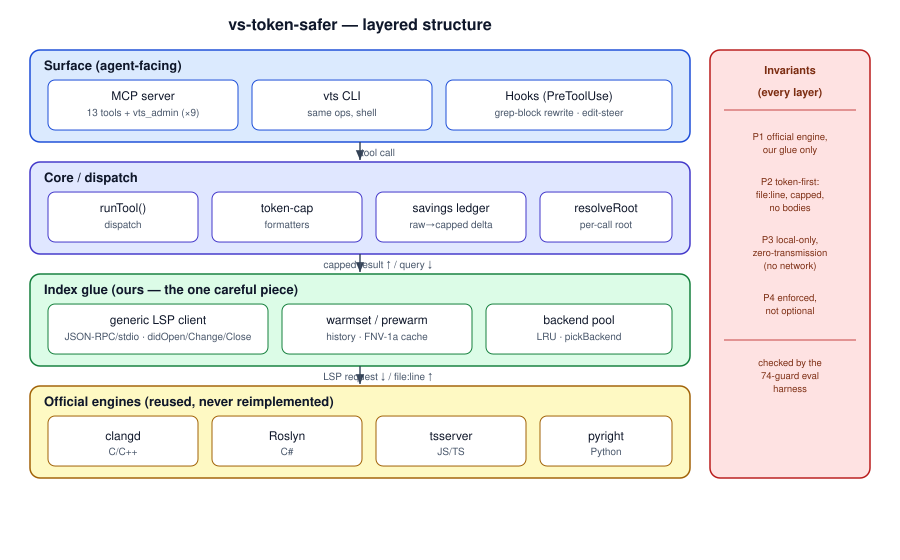
\includegraphics[width=0.96\linewidth]{figures/layers.pdf}
\caption{에이전트 표면부터 공식 엔진까지의 네 계층과, 모든 계층이 준수해야 하고 하버스가
검사하는 네 불변식(P1--P4). 본 연구가 구현하는 계층은 인덱스 접착부뿐이며, 엔진은 그대로
재사용한다.}
\label{fig:layers}
\end{figure}

\begin{figure}[h]
\centering
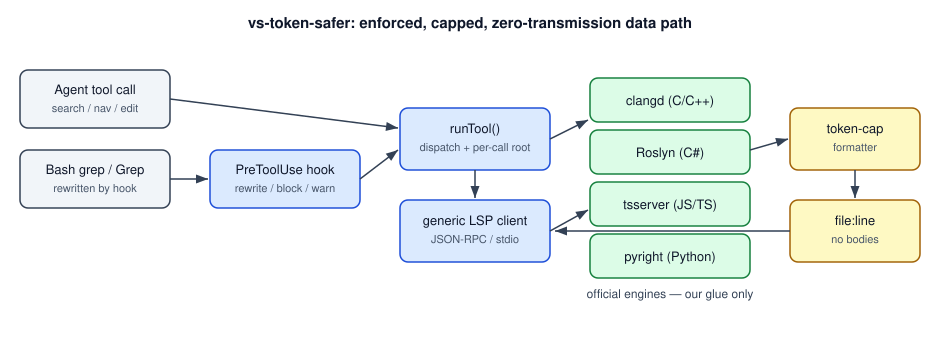
\includegraphics[width=\linewidth]{figures/architecture.pdf}
\caption{요청 경로. 도구 호출과 재작성된 grep은 단일 \texttt{runTool} 디스패치로 진입하고,
디스패치는 대상 파일의 공식 언어 서버 위로 범용 LSP 클라이언트를 구동한다. 포매터는 답을
\texttt{file:line} 목록으로 캡한 뒤 모델에 전달한다. 어떤 것도 호스트를 떠나지 않는다.}
\label{fig:arch}
\end{figure}

\subsection{범용 LSP 클라이언트}
유일하게 새롭고 섬세한 부품은 범용 JSON-RPC/stdio LSP 클라이언트이다. 두 동작이 중요하다.

첫째는 열기-또는-갱신 문서 동기화이다. 파일을 처음 참조하면 버전 1로 \texttt{didOpen}을
전송한다. 이미 열린 파일을 다시 참조하면 버전을 올린 \texttt{didChange}에 현재 디스크 텍스트를
실어 전송하므로, 워밍업 이후 가한 수정이 낡은 버퍼로 응답되지 않는다. 삭제된 파일은
\texttt{didClose}를 전송한다. 위치 기반 도구는 질의 전에 다시 열어, 호버·정의이동·아웃라인·
이름변경이 항상 현재 파일을 읽는다.

둘째는 서버 요청에 대한 규격 준수 응답이다. 서버 또한 클라이언트에 요청을 보내며, 이에 형태가
맞는 답을 반환한다. \texttt{workspace/configuration}에는 배열,
\texttt{workspace/applyEdit}에는 \texttt{\{applied:false\}} 등이다. 시간이 초과된 요청에는
\texttt{\$/cancelRequest}를 뒤따르고, 모르는 메서드에는 \texttt{MethodNotFound}를 반환한다.
사소한 세부이지만, 실제 언어 서버가 정지하지 않도록 유지하는 요소이다.

\subsection{혼합 저장소의 백엔드 선택}
저장소는 흔히 둘 이상의 언어를 포함하므로 백엔드는 질의마다 선택한다. 탐지는 가장 강한 빌드
산출물을 우선한다. 순서는 \texttt{compile\_commands.json} $\rightarrow$ clangd,
\texttt{.sln}/\texttt{.csproj} $\rightarrow$ Roslyn,
\texttt{tsconfig}/\texttt{package.json} $\rightarrow$ TypeScript,
\texttt{pyproject}/\texttt{*.py} $\rightarrow$ pyright이다.

특정 파일을 지명한 질의는 그 순서를 덮고 파일 확장자로 먼저 라우팅한다. 이 단일 규칙은 C++
루트 트리 내부의 \texttt{.py}나 \texttt{.ts} 파일이 clangd로 전달되어 아무것도 찾지 못하고
에이전트가 도구를 포기하게 되는 상황을 방지한다.

전역 설치된 단일 서버는 가장 가까운 프로젝트 표지까지 거슬러 올라가 호출별 루트를 결정하며,
따뜻한 백엔드의 LRU 풀(기본 상한 2, 유휴 클라이언트는 5분 후 회수)로 상주 메모리를 제한한다.

\subsection{워밍셋과 사전 워밍}
언어 서버가 비동기로 인덱싱하므로 첫 질의는 콜드 지연이 지배한다. 이에 \texttt{vts}는 서버의
열림 집합을 질의 가능성이 높은 방향으로 유도한다.

사전 워밍 후보는 이전 질의 이력, 현재 편집 중인 파일(\texttt{git status}나 Perforce
\texttt{opened}), 최근 git-log 파일, 인클루드 그래프 중심성, 수정 시각 순으로 정렬된다.

인클루드 그래프 캐시는 수정 시각·크기·FNV-1a 콘텐츠 해시의 합성 키를 사용한다. 따라서
타임스탬프가 흔들려도 바이트가 동일하면 캐시를 재사용하되, 타임스탬프만 사용하는 키가 놓칠
실제 수정은 포착한다. 언어별 워밍 상한은 각 언어의 파일 수에 비례하므로, 혼합 언어 저장소는
구성비에 비례하여 따뜻해진다.

\section{토큰 캡과 출력 압축}
\label{sec:cap}

토큰 이득은 시맨틱 질의의 선택이 아니라 포매터에서 발생한다. 세 전략이 작동한다.

\emph{본문이 아닌 위치.} 답은 \texttt{file:line}이며, 본문은 에이전트가 명시적으로 요청할
때만 읽는다. 편집조차 심볼 이름으로 제공한다(절~\ref{sec:beyond}).

\emph{반복 접기.} 참조가 많은 답은 파일별로 묶어 한 줄에 줄 번호를 모으고 중복 제거·정렬한다
(\texttt{Foo.cpp:42,88,120}). 이어 공통 디렉터리 접두사를 한 번만 추출한다. 모든 위치는
접두사와 꼬리로 복원 가능하다. 깊은 참조 결과에서 이 효과는 묶기로 약 $4\times$, 접두사
제거로 약 $10\times$까지 누적된다.

\emph{아웃라인 잡음 억제.} 문서 아웃라인은 익명 콜백과 중첩 지역 변수를 기본으로 숨기고 선언
구조와 숨긴 개수를 남긴다. 한 사례에서 105개 심볼 아웃라인이 보이는 항목 32개로 감소하였다.

\emph{캡 이전 재랭킹.} 캡은 상위 N개 행만 남기므로, 그 순서가 모델이 원하는 행이 표시되는지를
좌우한다. 따라서 캡 이전에 엔진의 결과를 재랭킹한다. 어휘 일치 품질(정확, 접두사, 단어·카멜
경계, 그다음 일반 부분 문자열), 호출 가능 종류에 대한 작은 선호, 그리고 사전 워밍에서 재사용한
질의 이력 신호를 사용한다. 이는 Semble~\cite{semble-hn}이 효과적이라 보고한 어휘+시맨틱 융합을
채택하되, 임베딩 벡터가 아니라 공식 엔진의 결과를 정렬하므로 인덱스를 추가하지 않고 아무것도
전송하지 않는다. \texttt{VTS\_RANK=0}으로 끌 수 있다.

확신 있는 랭킹은 한 걸음 더 나아가게 한다. 큰 결과 집합에 정확한 이름 일치가 나타나면 ---
알려진 심볼 하나를 찾는 흔한 경우 --- 전체 캡 대신 그것과 이웃 몇 개만 보이고, 나머지는 초과
주석과 복구 파일에 남긴다(\texttt{VTS\_FOCUS=0}으로 전체 목록 복원). 그리고 여러 단어 질의에
대해 \texttt{search\_text}는 질의의 용어를 몇 개나 담는지로 줄을 정렬한다. 임베딩이 필요 없는
개념 검색의 어휘적 근사이다(\texttt{VTS\_CONCEPT=0}으로 끔). 시맨틱한 동의어 인식 개념 검색은
임베딩을 요구하므로, 저장 인덱스를 거부하는 같은 규칙에 따라 범위 밖에 둔다.

답이 캡되면 \texttt{vts}는 질의를 재실행하지 않고 전체 집합을 복구하도록 ``tee'' 파일을
기록한다. 절감 원장은 도구별 원시-대-캡 토큰 차이를 기록하며, 절~\ref{sec:eval}이 그 원장을
읽는다.

\section{행동 강제}
\label{sec:enforce}

훅은 \texttt{Bash} grep 계열 명령(grep·rg·ack·ag·findstr·\texttt{git grep}·
\texttt{find -name})과 내장 Grep·Glob 도구를 가로챈다.

\paragraph{차단이 아닌 재작성.}
안전한 단일 grep 세그먼트는 사전 훅의 입력 변형 채널을 통해 동일 의미의 \texttt{vts} CLI
호출로 재작성된다. 결과는 토큰캡되고 에이전트의 흐름은 끊기지 않는다.

세그먼트 분리기는 따옴표를 인식하여, 따옴표 내부의 \texttt{|}를 셸 파이프가 아닌 정규식 교대로
해석한다. 그 결과 가장 흔한 두 우회인 \texttt{grep "FooA|FooB"}와
\texttt{grep "\^{}\#include"}가 토큰캡 텍스트 검색으로 정확히 재작성된다. 모호하거나 안전하지
않은 명령(실제 파이프, 위험한 패턴, 루트 경로 내 따옴표)만 강한 차단으로 후퇴하며, 이때도 즉시
실행 가능한 대체를 출력한다.

\paragraph{심볼 사냥 분류.}
심볼을 명백히 열거하는 grep은 시맨틱 심볼 검색으로 라우팅된다. 그 단서는 맨 식별자,
\texttt{::}나 리터럴 \texttt{(}나 타입 키워드 같은 코드 구조 단서를 포함한 정규식, 또는
\texttt{MaxWalkSpeed|MaxExcessSpeed} 같은 CamelCase·스네이크 교대이다.

식별자 신호가 없는 키워드 교대, 예를 들어 \texttt{TODO|FIXME}나 \texttt{GET|POST}는 거짓
양성을 피하기 위해 경고로 남긴다. 모든 강제는 탈출구 환경 변수로 되돌릴 수 있으며, 메시지는
운영자 로케일로 출력된다.

\paragraph{편집 습관 측정과 유도.}
우회는 검색에 국한되지 않는다. 두 번째 우회는 \emph{선언 전체}를 교체·삽입하는 내장 줄 기반
편집이다. 이는 심볼 단위 편집이라면 파일을 컨텍스트로 먼저 읽지 않고 이름만으로 수행할 수 있는
작업이다.

오프라인 발견 스캔과 라이브 훅이 공유하는 분류기가 그러한 편집을 표시한다. 선언처럼 보이는
제어 흐름 블록은 제외하며, 심볼 편집이라면 건너뛰었을 사전 파일 읽기 토큰을 귀속한다.

이어 세 계층이 습관 전환을 시도한다. 검색 결과에 얹은 집중 유도, 즉시 실행 가능한 심볼 편집
호출을 실은 모델 가시 경고, 그리고 안전한 삽입에 대한 옵트인 1회 차단이다. 채택 원장은 현재
채택 비율을 세션 목표로 재주입하는데, 이는 정적 지시가 제공할 수 없는 측정-후-재주입 루프이다.
이 습관의 완강함은 절~\ref{sec:discuss}에서 보고한다.

\section{검색을 넘어: 탐색·호출 계층·편집·시각화}
\label{sec:beyond}

동일한 캡·무전송 규율이 참조 검색 너머로 확장된다.

\paragraph{접힌 탐색.}
\texttt{goto\_definition}은 새 도구를 추가하는 대신 \texttt{kind} 매개변수 뒤로 타입 정의·
구현·선언을 접는다. 호버, 문서 심볼, 그리고 \texttt{file:line:col severity [code]: msg}
형태로 렌더된 간결한 진단 목록이 읽기 표면을 완성한다.

\paragraph{도구가 아닌 접힘으로서의 호출 계층.}
다중 홉 호출 계층, 즉 편집 전 영향 반경을 이루는 추이적 호출자 또는 피호출자는
\texttt{direction} 매개변수로 참조 도구 \emph{안에} 접힌다. 이는 순환·깊이 가드(기본 깊이 5,
노드 80)와 함께 공식 LSP \texttt{callHierarchy} 요청 위에서 구현된다. 영속 호출 그래프의
주문형 대응물로서, 실제 시맨틱 간선을 제공하되 저장된 그래프가 없고, 전송이 없으며, 표면에 새
도구가 없다.

\paragraph{심볼 단위 편집.}
본문 교체, 앞/뒤 삽입, 참조 검사 안전 삭제는 각각 LSP 아웃라인으로 선언을 이름으로 해석하여
심볼 구간에서 텍스트를 이어 붙인다. 모두 기본이 미리보기이며, 안전 삭제는 심볼이 아직 참조되는
동안에는 강제하지 않는 한 거부한다. 심볼을 이름으로 지정하는 편집은 파일 전체를 읽고 정확
일치를 위해 줄을 세는 작업을 건너뛰므로, 검색 캡의 편집 대응물이다.

\paragraph{로컬·무전송 시각화.}
옵트인·CLI 전용 대시보드는 번들된 동일 출처 WebGL 라이브러리(CDN 없음)로 인클루드 그래프와
주문형 호출 그래프를 3D로 렌더한다. 루프백에만 바인딩되며 MCP 서버는 이를 절대 기동하지 않는다.
헌장의 시각화 대응물로서, 유용한 뷰를 제공하되 호스트를 떠나는 것은 없다.

\section{평가}
\label{sec:eval}

본 연구는 세 축으로 평가한다. 결정적 회귀 하버스, 실제 프로젝트에서의 라이브 언어 서버 검증,
그리고 수 개월의 단일 개발자 사용 데이터이다.

구분은 의도적이다. 하버스는 통제되고 재현 가능하다. 사용 데이터는 실사용이므로 통제된
벤치마크가 아니라 관측이다. 답 품질의 다중 저장소 A/B 연구를 주장하지 않는다. 캡이 유지되고,
강제가 발동하며, 실현된 절감이 측정 가능하다는 것을 주장한다.

\subsection{회귀 하버스}
모의-LSP 하버스(\texttt{eval/run.mjs})는 툴체인 없이 모든 도구와 불변식을 실행한다. 토큰 캡
동작, 백엔드 선택, 문서 동기화 신선도, 강제 재작성, 그리고 새 기능 각각을 검증한다.

하버스는 현재 \textbf{74개 검사}를 포함하고 전부 통과한다. 모든 새 코드 경로는 검사와 함께
도입되며, 이는 원칙 P2의 운영 형태이다. 한 구체 수치로, 원시 인덱스 응답이 약 $57{,}308$
토큰인 콜드 작업공간-심볼 질의는 약 $1{,}434$ 토큰으로 캡되어 대략 $40\times$ 감소한다.

\subsection{라이브 언어 서버 검증}
네 백엔드 각각을 모의가 아닌 공식 엔진에 대해 끝까지 검증하였다.

\begin{itemize}
  \item \textbf{C/C++ (clangd)} 실제 Unreal Engine 5.x 프로젝트에서
  \texttt{search\_symbol}이 게임 \texttt{UCLASS}와 그 생성 심볼을 \texttt{file:line}으로
  반환하였다. 재현 가능한 사실 둘이 도출되었다. 첫째, 타깃이 clang-cl로 빌드되면
  \texttt{GenerateClangDatabase}에 \texttt{-Compiler=VisualCpp}가 필요하다. 둘째, 번들
  clangd 19.1.5는 서버 모드에서 전체 게임 번역 단위에 데드락하지만, 독립 clangd $\geq 22$는
  같은 단위를 약 13초에 파싱한다. 이에 버전을 탐지하고, 찾는 심볼의 샤드가 로드되는 순간
  응답하는 영속-인덱스 빠른 경로를 사용한다. 이 경로는 전체 백그라운드 인덱스를 기다리는
  $369$초를 정적 인덱스 로드 후 $51$초로 전환하며, 첫 질의 지연을 $7\times$ 단축한다.
  \item \textbf{C\# (Roslyn 기반 서버)} Microsoft.CodeAnalysis.LanguageServer(Visual
  Studio·C\# Dev Kit 엔진)에 대해 검증하였다.
  \item \textbf{JS/TS (\texttt{typescript-language-server})} \texttt{vts}를 자체 소스에
  실행하여 검증하였다.
  \item \textbf{Python (pyright)} TypeScript와 동일한 범용 접착부로 검증하였다.
\end{itemize}

\subsection{토큰 절감 데이터}
단일 개발자의 기록된 $441$회 검색에서, 로컬 원장은 캡 출력을 원시 인덱스 응답보다 약
$2\times$ 작게 기록한다. $263{,}540$ 토큰이 $133{,}289$로 감소하여 약 $130{,}000$ 토큰을
절감하였다. 가장 무거운 단일 질의는 $21{,}056$에서 $1{,}961$ 토큰으로 $10.7\times$ 압축된다.

그림~\ref{fig:savings}과 표~\ref{tab:savings}이 절감을 도구별로 분해한다. 문서 아웃라인
억제와 텍스트 검색 캡이 절감을 지배한다.

이 수치는 검색 결과 자체의 압축만 센다. 더 크고 측정하기 어려운 절반 --- 에이전트가 파일을
열지 않게 되어 절약한 읽기 --- 은 빠져 있다. 에이전트가 \texttt{file:line} 위치와 이름 지정된
심볼 span을 받기 때문이다. 그 읽기 회피의 일부를 \texttt{read\_symbol}을 그것이 대체하는 전체
파일 대비로 측정하여 원장에 드러낸다. 이는 Semble이 절감을 ``파일 읽기와 결합하여'' 보고하는
방식과 같다~\cite{semble-hn}.

\begin{figure}[h]
\centering
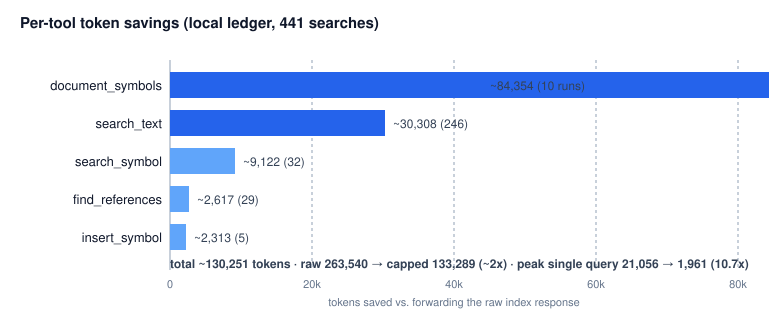
\includegraphics[width=0.92\linewidth]{figures/savings.pdf}
\caption{로컬 원장의 도구별 토큰 절감(441회 검색, 개발자 1인). 통제된 벤치마크가 아닌 관측
사용 수치이다.}
\label{fig:savings}
\end{figure}

\begin{table}[h]
\centering
\caption{로컬 원장의 도구별 토큰 절감. 관측 데이터.}
\label{tab:savings}
\begin{tabular}{lrr}
\toprule
도구 & 실행 & 절감 토큰 \\
\midrule
\texttt{document\_symbols} & 10  & $\sim$84{,}354 \\
\texttt{search\_text}      & 246 & $\sim$30{,}308 \\
\texttt{search\_symbol}    & 32  & $\sim$9{,}122 \\
\texttt{find\_references}  & 29  & $\sim$2{,}617 \\
\texttt{insert\_symbol}    & 5   & $\sim$2{,}313 \\
\midrule
\textbf{vts 합계}          & 441 & $\sim$130{,}251 \\
\bottomrule
\end{tabular}
\end{table}

\subsection{강제 커버리지}
에이전트 자신의 세션 기록을 훑는 오프라인 발견 스캔이 얼마나 많은 코드 검색이 \texttt{vts}를
우회했는지 측정한다. 대형 게임 엔진 작업부하에서 매처의 최근 구간 포착률은 약 $68\%$이다.

심볼 사냥 grep을 겨눈 두 강제 개선은 잠재 우회 중 월 약 $172$k 토큰(구조적 grep 차단)과 추가
$319$k 토큰(CamelCase 교대 grep 차단)을 가로채는 것으로 관측된다.

같은 스캔이 편집 습관을 정량화한다. 30일 동안 $1{,}284$건의 선언 전체 줄 편집이 약 $468$k
토큰의 파일 내용을 먼저 읽었으며, 그중 $93\%$는 그 파일에 대한 사전 \texttt{vts} 검색 없이
발생하였다. 이 수치는 검색 결과만으로 수행하는 유도의 기회와 천장을 동시에 측정하며, 편집 채택
원장이 존재하는 이유이다.

\subsection{타당성 위협}
위협을 명시한다.

\emph{외적 타당성.} 절감·강제 데이터는 한 개발자, 한 환경에서 도출되었으므로 절댓값은 효과의
존재 증명이지 모집단 추정이 아니다. 코드 구성이나 작업 방식이 다르면 값도 달라진다.

\emph{구성 타당성.} 토큰은 원시 인덱스 응답 대비로 측정하므로 형식 이득은 포착하지만,
에이전트가 grep으로 도달했을 답에 동일하게 도달했는지는 포착하지 않는다. 정확성은 시맨틱 엔진의
사용과 라이브 검증에서 주장하며, 작업 성공 지표로 주장하지 않는다.

\emph{내적 타당성.} 원장은 측정 대상과 동일한 프로세스의 계측이며, 입력 하나(번들 로그 압축
항목)는 비정상이므로 결합 대신 분리하여 보고한다.

\emph{참고문헌 품질.} 관련 연구의 일부는 동료 심사 지면이 아닌 현장 글을 인용하는데, 이는
에이전트-LSP 전환이 최근이기 때문이다. 그러한 출처는 그대로 표시하고, 핵심 주장을 거기에 싣지
않는다.

\subsection{아티팩트 가용성}
\texttt{vs-token-safer}는 설치 가능한 MCP 플러그인과 CLI로 배포되며, 본 절의 평가는
저장소에서 재현된다. \texttt{node eval/run.mjs}는 툴체인 없이 74개 검사를 실행하고,
\texttt{vts savings}는 표~\ref{tab:savings}의 바탕 원장을 출력한다.

본 논문의 도표는 버전 관리되는 SVG 소스에서 생성된다(\texttt{figures/build.py}). 여기 수치는
릴리스 v0.32.2 기준이며, 원장이 사용에 따라 증가하므로 정확한 값을 인용하기 전에 두 명령을 다시
실행하고 재빌드할 것을 권한다.

\section{논의와 한계}
\label{sec:discuss}

\paragraph{grep이 남는 영역.}
\texttt{vts}는 어휘 검색을 폐지하지 않고 제한한다. 언어 서버는 그것이 존재하는 형식에만 있는
반면, 에이전트의 검색 수요는 트리의 모든 텍스트를 포괄한다.

따라서 \texttt{vts}는 형식 무관 경우를 위해 토큰캡 텍스트 검색 도구를 유지하고, 시맨틱 답이
엄밀히 더 나은 경우(심볼 사냥, 참조, 이름변경)에만 강제를 적용한다. 자유형과 키워드 교대 검색은
의도적으로 경고로 둔다.

\paragraph{콜드 지연.}
실제 컴파일러 프런트엔드를 사용하는 정직한 대가는 콜드·대형 인덱스의 첫 질의 지연이다.
\texttt{vts}는 사전 워밍, 영속-인덱스 빠른 경로, 샤드 로드까지의 폴링으로 이를 완화하지만
제거하지는 못한다. 이미 실행 중인 언어 서비스를 프록시하는 따뜻한 IDE는 여전히 첫 질의에 더
빠르게 응답한다. 서버를 상주시키면 적어도 스폰 비용을 호출마다가 아니라 세션마다 한 번 지불한다.

\paragraph{채택은 기술이 아니라 행동 문제이다.}
가장 두드러진 측정 격차는 도구의 능력이 아니라 에이전트가 그것을 사용하는지이다. 캡된 심볼
편집이 존재해도 에이전트는 여전히 열에 아홉은 줄 기반 편집을 기본으로 선택한다.

영구 강제 차단은 역효과였다. 에이전트를 우회 시도의 반복에 가두기 때문이다. 수치를 실제로
움직인 지렛대는 즉시 실행 가능한 제안 호출과 재주입된 라이브 채택 지표였다. 이 격차의 축소가
본 연구가 가장 중시하는 미해결 문제이다.

\paragraph{평가의 정직함.}
정량 결과는 사용 데이터와 결정적 하버스이지, grep이나 영속 지식 그래프에 대한 답 품질의 통제된
다중 저장소 벤치마크가 아니다. 자연스러운 다음 단계가 그 연구이다. 에이전트와 작업을 고정하고
검색 백엔드만 변경하여, 저장소 모음에 걸쳐 토큰·실시간·작업 성공을 측정한다. 현 데이터를
부풀리는 대신 향후 과제로 명시한다.

\section{결론}
\label{sec:conc}

\texttt{vs-token-safer}는 에이전트의 코드 검색을 시맨틱하고, 캡되고, 무전송이며, 강제되게
만든다. 공식 언어 서버를 분석 엔진으로 재사용하고 LSP-MCP 접착부만 구현한다. 본문이 아니라
위치를 반환하고, grep을 훅에서 동일 의미의 캡 호출로 재작성한다. 이로써 탐색·참조·이름변경
계열 연산의 토큰·프라이버시 비용을 낮추되, 어휘 검색은 적합한 영역에 남긴다.

영속 지식 그래프와 비교하면, \texttt{vts}는 저장 인덱스의 도달 범위와 언어 폭을 구성에 의한
정확성(컴파일러 자신의 프런트엔드), 무효화 문제 없는 신선도, 단단한 무전송 보장과 맞바꾼다.

남기는 문제는 기술이 아니라 행동이다. 에이전트가 더 저렴한 도구를 사용하게 만드는 것이며,
거기에서는 영구 차단보다 라이브 측정과 재주입이 더 효과적이었다.

% ============================================================================
\begin{thebibliography}{9}

\bibitem{cbm}
DeusData.
\newblock Codebase-Memory: Tree-Sitter-Based Knowledge Graphs for LLM Code
Exploration via MCP.
\newblock arXiv:2603.27277, 2026. \url{https://arxiv.org/abs/2603.27277}

\bibitem{anthropic-lsp}
Anthropic.
\newblock Native Language Server Protocol support in Claude Code (v2.0.74),
December 2025.

\bibitem{lsp-medium}
V.\ Thiagarajan.
\newblock LSP --- The Protocol Your IDE Uses Every Day (And Now Your AI Agent
Does Too). Medium, 2026.

\bibitem{semble-hn}
Semble.
\newblock Code search for agents that uses 98\% fewer tokens than grep.
Hacker News, 2026. \url{https://news.ycombinator.com/item?id=48169874}

\bibitem{yage-grep}
Yage.
\newblock Why Coding Agents Still Use grep as Their Search Backbone. 2026.
\url{https://yage.ai/share/why-coding-agents-still-use-grep-en-20260327.html}

\bibitem{hyperagent}
H.\ N.\ Phan, T.\ N.\ Nguyen, P.\ X.\ Nguyen, and N.\ D.\ Q.\ Bui.
\newblock HyperAgent: Generalist Software Engineering Agents to Solve Coding Tasks
at Scale.
\newblock arXiv:2409.16299, 2024.

\end{thebibliography}

\end{document}
